\documentclass[10pt] {article}
\usepackage{fullpage}
\usepackage{amssymb}
\usepackage{graphicx}
\usepackage{float}
\usepackage{amsthm}
\usepackage{hyperref}
\usepackage{amsmath}
\renewcommand\qedsymbol{$\blacksquare$}

\title{Homework 2 }
\author{Ricky Hempel}
\begin{document}
\maketitle
\begin{center}
1.6 a-i, k, m-n, 1.7
\end{center}
\begin{enumerate}
\item[1.6]
a.
\begin{figure}[H]
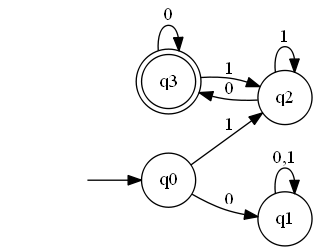
\includegraphics[width=0.4\textwidth]{a6.png}
\caption{ State diagram for a.}
\label{8}
\end{figure} 
b.
\begin{figure}[H]
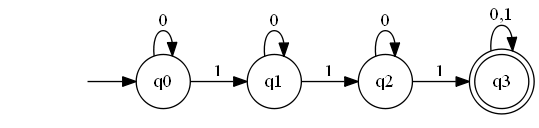
\includegraphics[width=0.6\textwidth]{b6.png}
\caption{State diagram for b.}
\label{8}
\end{figure} 
c.
\begin{figure}[H]
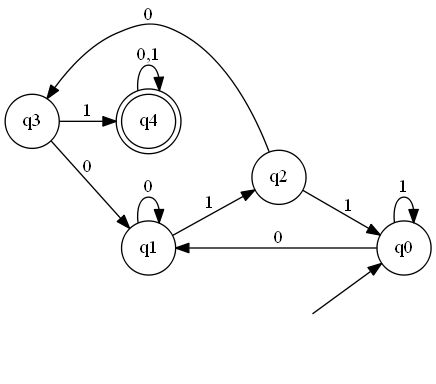
\includegraphics[width=0.5\textwidth]{c6.png}
\caption{State diagram for c.}
\label{8}
\end{figure} 
d.
\begin{figure}[H]
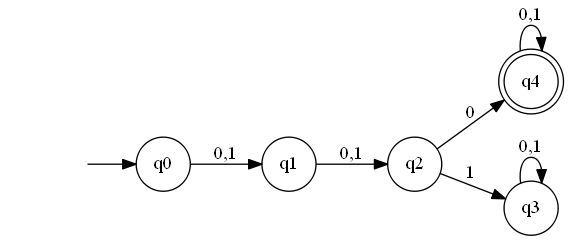
\includegraphics[width=0.6\textwidth]{d6.png}
\caption{State diagram for d.}
\label{8}
\end{figure} 
e.
\begin{figure}[H]
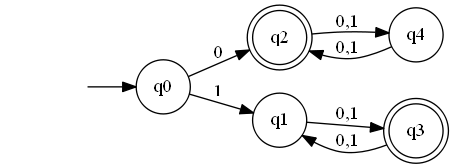
\includegraphics[width=0.6\textwidth]{e6.png}
\caption{State diagram for e.}
\label{8}
\end{figure} 
f.
\begin{figure}[H]
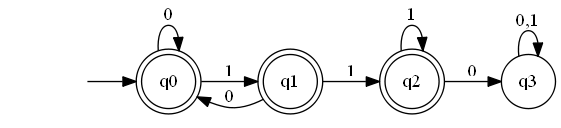
\includegraphics[width=0.6\textwidth]{f6.png}
\caption{State diagram for f.}
\label{8}
\end{figure} 
g.
\begin{figure}[H]
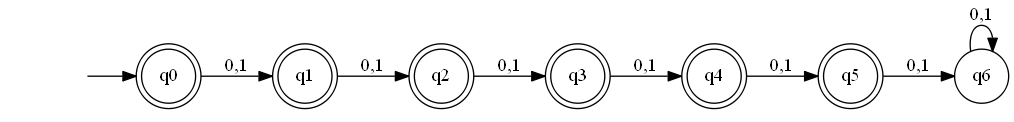
\includegraphics[width=1.1\textwidth]{g6.png}
\caption{State diagram for g.}
\label{8}
\end{figure} 
h.
\begin{figure}[H]
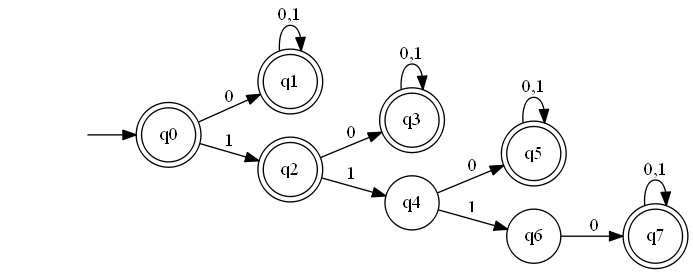
\includegraphics[width=0.9\textwidth]{h6.png}
\caption{State diagram for h.}
\label{8}
\end{figure} 
i.
\begin{figure}[H]
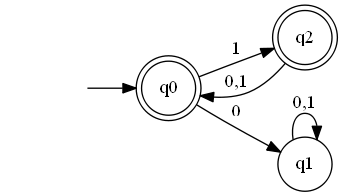
\includegraphics[width=0.5\textwidth]{ii6.png}
\caption{State diagram for i.}
\label{8}
\end{figure}
k.
\begin{figure}[H]
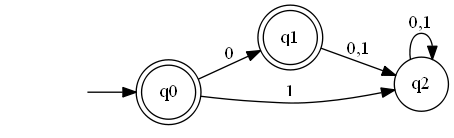
\includegraphics[width=0.6\textwidth]{kk6.png}
\caption{State diagram for k.}
\label{8}
\end{figure}
m.
\begin{figure}[H]
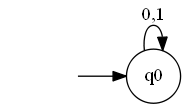
\includegraphics[width=0.4\textwidth]{m6.png}
\caption{State diagram for m.}
\label{8}
\end{figure}
n.
\begin{figure}[H]
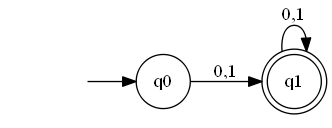
\includegraphics[width=0.4\textwidth]{n6.png}
\caption{State diagram for n.}
\label{8}
\end{figure}
\item[1.7]
a.
\begin{figure}[H]
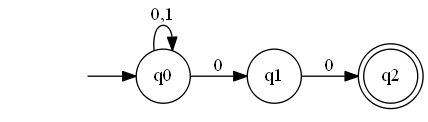
\includegraphics[width=0.8\textwidth]{a7.png}
\caption{ State diagram for a.}
\label{8}
\end{figure}
b.
\begin{figure}[H]
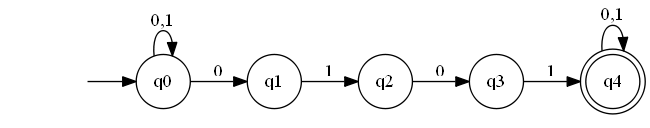
\includegraphics[width=0.8\textwidth]{b7.png}
\caption{State diagram for b.}
\label{8}
\end{figure}
c.
\begin{figure}[H]
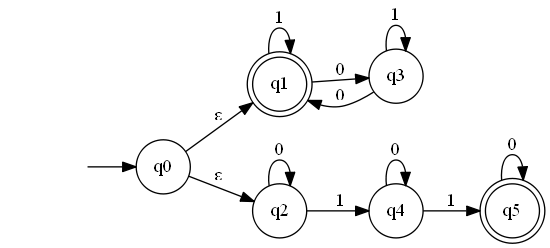
\includegraphics[width=0.8\textwidth]{c7.png}
\caption{State diagram for c.}
\label{8}
\end{figure} 
d.
\begin{figure}[H]
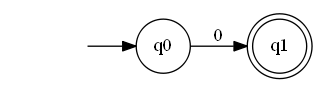
\includegraphics[width=0.8\textwidth]{d7.png}
\caption{State diagram for d.}
\label{8}
\end{figure} 
e.
\begin{figure}[H]
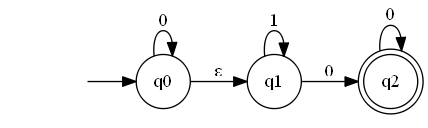
\includegraphics[width=0.8\textwidth]{e7.png}
\caption{State diagram for e.}
\label{8}
\end{figure} 
f.
\begin{figure}[H] 
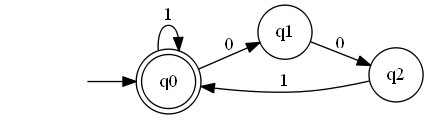
\includegraphics[width=0.8\textwidth]{f7.png}
\caption{State diagram for f.}
\label{8}
\end{figure} 
g.
\begin{figure}[H]
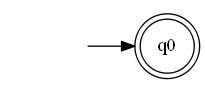
\includegraphics[width=0.4\textwidth]{g7.png}
\caption{State diagram for g.}
\label{8}
\end{figure} 
h.
\begin{figure}[H]
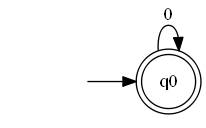
\includegraphics[width=0.4\textwidth]{h7.png}
\caption{State diagram for h.}
\label{8}
\end{figure} 
\end{enumerate}
\end{document}
